\documentclass[a4paper,twocolumn]{article}
\usepackage[utf8]{inputenc}
\usepackage{amsmath}
\usepackage{amsfonts}
\usepackage{amssymb}
\usepackage{tikz}
\usepackage{hyperref}
\usepackage{url}
\usepackage{paralist}
\usepackage[left=2cm,right=2cm,top=2cm,bottom=2cm]{geometry}
\RequirePackage[date=terse,isbn=true,doi=true,url=false,maxbibnames=9,backref=false]{biblatex}
\addbibresource{securityupdates.bib}
\renewcommand{\bibfont}{\small}

\AtEveryBibitem{% Clean up the bibtex rather than editing it
 \clearname{editor} % remove editors
}

\author{Daniel Thomas}
\title{Android security updates: late or never}
\date{}%no date, it takes up space
\begin{document}
\maketitle

\section*{Problem definition}
I am working on improving the security of Internet of Things (IoT) devices, looking at both secure synchronisation of data and the security of the underlying device operating system.

The Internet of Things means that there will be many more internet connected devices, which will run complex software.
Security vulnerabilities will be found in this software which will then need to be updated.
Android is one operating system which is being used for Internet of Things devices (fridges, toasters etc.) and so examining the trends in security updates for Android gives us insight into how updates for Internet of Things devices might evolve.
Our preliminary results indicate that most Android devices do not receive security updates in a timely manner.
Android devices are user facing and probably more likely to receive updates than fridges or water meters so the situation is likely to be worse in the IoT.
I intend to quantify this and compare different manufacturers to determine which are the best at shipping security updates promptly.
Initial analysis indicates that perhaps the Qualcomm Innovation Center, Inc. (QuIC) is the best at following best practice and making patches available~\cite{codeaurora-security-advisories} and Google the fastest at shipping updates to devices promptly.
However I do not yet have sufficient data to make robust conclusions.


\section*{Innovation proposal}
Presently there is not much visibility into the impact of security vulnerabilities on Android, many root equivalent vulnerabilities do not have CVEs registered even when they are being actively exploited.
It is also difficult to determine when vulnerabilities have been fixed and these fixes propagated to users.
I have started the Android Vulnerabilities website~\cite{androidvulnerabilities.org} to collate such information, particularly on root equivalent vulnerabilities.
The current database is publicly available in a machine readable format (JSON) and the code is open source.
Root equivalent vulnerabilities are vulnerabilities which can be exploited either to gain root or to gain privileges which can then be used to either gain root on the device or do things which only root would normally be able to do.
By using the database of root equivalent vulnerabilities that I have collected, together with the data we have collected with Device Analyzer (DA)~\cite{Wagner2013} we can start to determine the proportion of devices running vulnerable versions of Android.
We can then chart how that changes over time as new vulnerabilities are discovered and old ones are fixed, this is shown in Figure \ref{fig:propinsecure}.

\begin{figure}
 \includegraphics[width=0.5\textwidth]{figures/proportioninsecure.pdf}
 \caption{Proportion of devices running vulnerable versions of Android}
 \label{fig:propinsecure}
\end{figure}

We have only just started and there is still much to do to improve the quantity and quality of the data so that it is useful.
We need a more representative coverage of root equivalent vulnerabilities on Android, currently we only have a subset with many important details missing from the ones which we have.
The improvement in the middle of Figure \ref{fig:propinsecure} might be due to not yet having sufficient data to include any of the vulnerabilities found in 2012 (we know of several).
In particular manufacturer specific flaws are under-represented and there are many details which need to be tracked down to improve the reliability of the results.
There is also information which is not presently publicly available but which it might be possible to ask manufacturers and those who found vulnerabilities for in order to get a better picture of what is actually happening.
Presently while we can chart the data we have, we cannot be sure that it is representative.

Existing databases such as the CVE database~\cite{cve-details} lack information vital to performing these sorts of analyses such as dates for discovery, and release dates for fixes.
Even finding release dates for Android versions is difficult as there is no canonical list.
For example: dates of tags in the Android Open Source Repository are unreliable indicators of release dates, sometimes being tagged well after devices have started receiving updates to that version.
Collating all the information together and checking its accuracy is a significant undertaking, the idea is to provide a good starting point and then use crowd-sourcing for the remainder once the Android Vulnerabilities website is a useful resource.
We have already started getting submissions from other people to improve it.

Once we can make accurate comparisons between manufacturers regarding the timeliness with which they ship security updates to customers then we can publish this information and hence create an incentive for manufactures to ship updates more promptly.
For example we could produce press releases or badges stating which companies are most prompt at shipping updates.
CESG which advises government on how to secure its computer system recommends picking Android devices from manufactures which are good at shipping security updates promptly~\cite{CESG2013} but it does not state which manufacturers are better.
Enterprises with Bring Your Own Device policies or which supply smartphones for work purposes are likely to also be interested in this information.
If an app can root a phone then any attempt to prevent data leakage are rendered useless.

We determine whether a particular device is vulnerable to a vulnerability by computing which versions of Android were vulnerable to that vulnerability on a particular day from the vulnerabilities database and comparing that with the proportion of devices running that version, this is shown in Figures \ref{fig:da_norm_os} and \ref{fig:norm_os_heat}.
They show how the distribution of versions changes with time and how the popularity of each version changes.

The variation of the proportion of devices affected by a vulnerability with time tells us how bad a particular vulnerability affected the Android platform.
Figure \ref{fig:nvulnerabilities_heat} breaks this down by vulnerability to show how the proportion of devices affected by different vulnerabilities varies.
In 2013 three vulnerabilities were found in the way which Android verified the signatures on APKs.
These allowed the creation of malicious APKs which appear to be signed as system APKs -- which have root equivalent privileges.
Figure \ref{fig:nvulnerabilities_heat} shows how the the \emph{APK signing vulnerabilities} affected all devices and took months to get fixed for any device.
However what is perhaps more worrying is the long tail on the \emph{Gingerbreak}, \emph{levitator} and \emph{exploid} vulnerabilities which are more dangerous root exploits (not requiring new APK installation) and which still affect a significant proportion of devices years later.

These graphs only show a small subset of the total vulnerabilities and only those which affect all Android devices, not any that are manufacturer or device specific.
Hence observations of the proportion of devices affected in total are underestimates.
\begin{figure}
 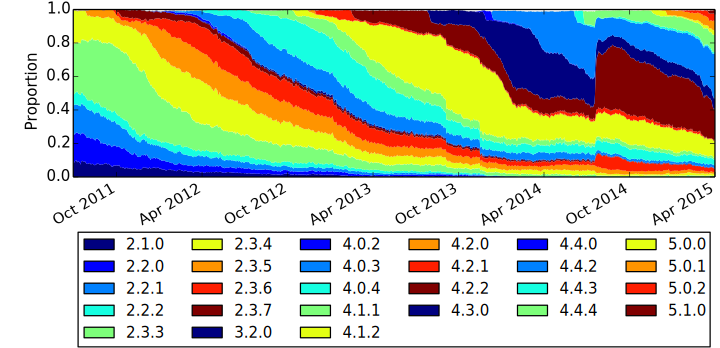
\includegraphics[width=0.5\textwidth]{figures/da_norm_os.pdf}
 \caption{Proportion of devices running different OS versions in the DA data (see also \ref{fig:norm_os_heat})}
 \label{fig:da_norm_os}
\end{figure}
\begin{figure}
 \includegraphics[width=0.5\textwidth]{figures/norm_os_heat.pdf}
 \caption{Proportion of devices running different OS versions in the DA data (see also \ref{fig:da_norm_os})}
 \label{fig:norm_os_heat}
\end{figure}
\begin{figure}
 \includegraphics[width=0.5\textwidth]{figures/nvulnerabilities_heat.pdf}
 \caption{Proportion of devices affected by different vulnerabilities}
 \label{fig:nvulnerabilities_heat}
\end{figure}

\begin{figure}
 \includegraphics[width=0.5\textwidth]{figures/from_to_updates.pdf}
 \caption{Updates between different Android versions in the DA data}
 \label{fig:from_to_updates}
\end{figure}
\begin{figure}
 \includegraphics[width=0.5\textwidth]{figures/w_security_updates.pdf}
 \caption{Number of updates each week which fixed or may have fixed security vulnerabilities}
 \label{fig:weekly_security_updates}
\end{figure}
Figure \ref{fig:from_to_updates} shows how devices upgrade between different versions of Android.
Device Analyzer (DA) observes upgrade events and the figure shows which versions a device is upgrading from and to.
Mostly the dark cells are above the diagonal and are upgrades.
While many upgrades are from one version to the next version there are also a fair number which skip a few versions.
Surprisingly there are also a small number of downgrade events when older versions of Android are installed on to devices.
Figure \ref{fig:weekly_security_updates} shows the number of devices getting security updates each week, blue shows updates which changed the Android version number from a version with known vulnerabilities to one which had fewer known vulnerabilities.
Red indicates updates which changed the build number but not the version number and so might contain a backported fix for a vulnerability.
We need better data to detect backporting of security fixes.

\section*{One year horizon}
\begin{itemize}
 \item A comprehensive database of root equivalent vulnerabilities affecting Android in a machine readable format on the website~\cite{androidvulnerabilities.org}.
 \item Comparison of different manufacturers to determine which is best at shipping updates for security vulnerabilities.
 \item Analysis of the behaviour of users with respect to Android updates -- how promptly do they get installed once made available.
 \item A paper publishing the results.
 \item Updates to Device Analyzer to support further collection of useful data.
 \item Crowd sourcing of data on Android vulnerabilities and disclosure practices.
 \item Badges or other useful feedback for manufacturers following best practice.
\end{itemize}


\section*{Conclusion}
We have collected some data on root equivalent vulnerabilities on Android and version information for deployed Android devices.
Preliminary results are interesting and with more and better data we should be able to make useful recommendations about which manufacturers are best at shipping security updates.
This in turn should incentivise manufactures to do a better job and so improve end user security.
Improvements in end user security should give users more confidence in using their devices and this confidence is vital if the Internet of Things is to work out.
We will hopefully also be able to analyse the incentives which have created the current situation and look at how those could be changed.


\printbibliography

\end{document}